
% ***************************************************** %
\chapter{Titolo breve}\label{ch:chap-name}
% ***************************************************** %

\lipsum[1]

Nell'articolo di~\textcite{provaBib} \lipsum[1][1-2]

Si veda la bellissima figura~\vref{fig:lorem3}.

\begin{figure}
\centering

\includegraphics[width=0.4\textwidth]{./Figures/img2.jpg}
\caption{Figura completamente a caso}
\label{fig:lorem3}
\end{figure}

\section{Titolo breve del paragrafo}

\lipsum[1]

\subsection{Titolo della dimensione che preferisci}

\lipsum[2]

\lipsum[3]

Dai uno sguardo alla tabella~\vref{tab:tab1}.

\begin{table}
\centering
\caption{Una tabella per comparare cose}
\label{tab:tab1}
\begin{tabular}{lp{0.35\textwidth}p{0.35\textwidth}}
\toprule
\textbf{Pippo} & \textbf{Pluto} & \textbf{Paperino} \\
\midrule
Primo & \lipsum[1][1] & \lipsum[1][3-4] \\
Secondo & \lipsum[1][1] & \lipsum[1][3-4] \\
Terzo & \lipsum[1][1] & \lipsum[1][3-4] \\
\bottomrule
\end{tabular}
\end{table}

\section{Sempre un titolo breve}

Nell'articolo di~\textcite{altroBib} \lipsum[3-4]

\subsection{Titolo del sottoparagrafo}

\lipsum[1]

Si veda a proposito la figura~\vref{fig:prova_fig}.

\begin{figure}
\centering
\includegraphics[page=1]{./Figures/Drawings/MyThesis-drawings}
\caption{Un esempio di \engemph{flow chart}}
\label{fig:prova_fig}
\end{figure}

\subsubsection{Titolo di un sottosotto paragrafo della dimensione che preferisci}

\lipsum[2]

\lipsum[3]

Si veda la tabella~\vref{tab:prova_tab}.

\begin{table}
\caption{Esempio di tabella con testo}
\label{tab:prova_tab}
\begin{tabularx}{\textwidth}{lX}
\toprule
\textbf{Una cosa} & \lipsum[1][1-4] \\
\textbf{Un'altra cosa} & \lipsum[2][1-4] \\
\bottomrule
\end{tabularx}
\end{table}

\subsection{Altro titolo di sottoparagrafo}

\lipsum[1]

\section{Adesso delle figure}

\lipsum[1][1-5] come si vede nella figura~\vref{fig:lorem1}.

\begin{figure}
\centering
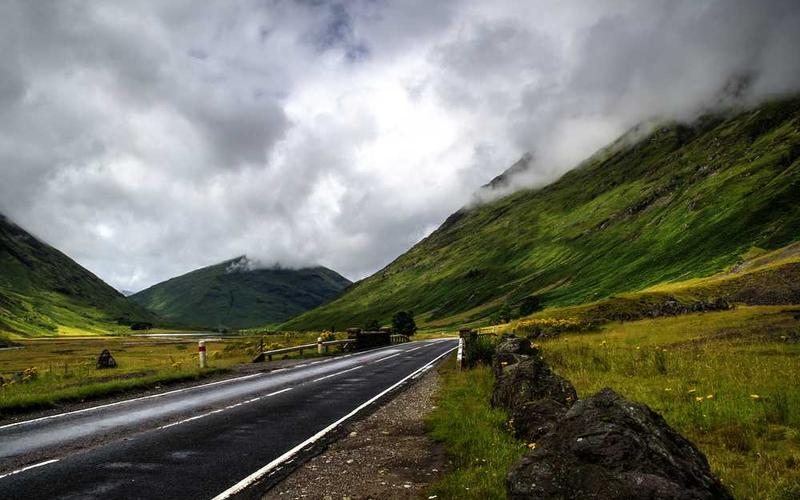
\includegraphics[width=\textwidth]{./Figures/img1.jpg}
\caption{Una figura \emph{lorem ipsum}}
\label{fig:lorem1}
\end{figure}

\lipsum[1][1-5]

\lipsum[1][1-5]

A tal proposito si vedano le figure~\ref{subfig:lorem2_1}~e~\vref{subfig:lorem2_2}.

\begin{figure}
\centering
\subfloat[][\emph{Didascalia di questa}\label{subfig:lorem2_1}]
	{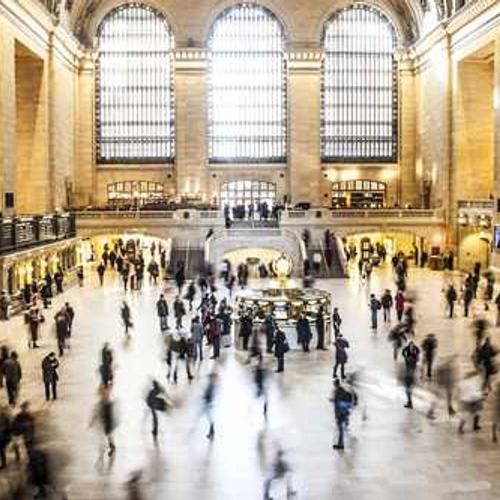
\includegraphics[width=0.45\textwidth]{./Figures/img3.jpg}} \quad
\subfloat[][\emph{Didascalia di quest'altra}\label{subfig:lorem2_2}]
	{
\includegraphics[width=0.45\textwidth]{./Figures/img4.jpg}}
\caption{Didascalia di un paio di figure a caso}
\label{fig:lorem2}
\end{figure}
